\chapter{Metodología y diseño experimental}

\section{Visión general del proyecto}

El objetivo principal de este trabajo es analizar de forma empírica cómo la complejidad del estado observado influye en el rendimiento de distintos algoritmos de Aprendizaje por Refuerzo. Para ello, se ha diseñado un marco experimental completo que abarca desde la creación de un entorno propio hasta la ejecución sistemática de entrenamientos, la optimización de hiperparámetros y la evaluación cuantitativa de los resultados obtenidos.

El proyecto se ha desarrollado siguiendo un enfoque modular y reproducible, apoyado en un repositorio de código que centraliza todos los componentes necesarios para la experimentación. Este repositorio incluye la definición del entorno, los scripts de entrenamiento para cada algoritmo, los procedimientos de evaluación, las herramientas de ajuste automático de hiperparámetros y los mecanismos de visualización del aprendizaje. Esta organización permite aislar responsabilidades, facilitar la replicabilidad de los experimentos y garantizar la trazabilidad de los resultados.

En primer lugar, se ha implementado desde cero un entorno de aprendizaje por refuerzo denominado \textit{SimplePacmanEnv}, inspirado en el clásico videojuego Pac-Man. Este entorno ha sido diseñado con el objetivo de permitir un control preciso sobre la información observacional proporcionada al agente, manteniendo constantes las dinámicas del juego y la función de recompensa. De este modo, es posible evaluar de manera aislada el impacto de diferentes configuraciones de estado sobre el proceso de aprendizaje.

Sobre este entorno se han entrenado agentes utilizando tres algoritmos representativos del Aprendizaje por Refuerzo Profundo: DQN, A2C y PPO. Cada algoritmo se ha entrenado mediante un script específico, garantizando una configuración homogénea del entorno y del protocolo de evaluación. Inicialmente, se llevaron a cabo múltiples ejecuciones exploratorias con ajustes manuales de hiperparámetros, lo que permitió adquirir una comprensión práctica del comportamiento de los algoritmos y de la sensibilidad del aprendizaje a distintos parámetros.

Posteriormente, y con el fin de sistematizar este proceso, se incorporó la librería Optuna para realizar la optimización automática de hiperparámetros. Esta herramienta permitió explorar de manera eficiente espacios de búsqueda amplios, reduciendo el sesgo introducido por la selección manual y mejorando la calidad de los modelos entrenados. Dada la elevada carga computacional asociada a estos experimentos, se definieron estrategias de compromiso entre exhaustividad y coste temporal, incluyendo criterios de parada temprana y frecuencias de evaluación ajustadas.

El rendimiento de los agentes entrenados se evaluó mediante un protocolo común basado en múltiples episodios de prueba, utilizando métricas cuantitativas como la recompensa media, la duración de los episodios y tasas de éxito. Adicionalmente, se emplearon herramientas de monitorización como TensorBoard para visualizar el progreso del aprendizaje y analizar de forma cualitativa el comportamiento de los agentes durante el entrenamiento.

En conjunto, este enfoque metodológico permite abordar de manera estructurada la pregunta de investigación planteada, proporcionando un marco experimental sólido para estudiar la relación entre la complejidad del estado y el rendimiento de los algoritmos de Aprendizaje por Refuerzo.

\section{Infraestructura del proyecto y repositorio}

Con el objetivo de garantizar la reproducibilidad, organización y trazabilidad de los experimentos, todo el desarrollo del proyecto se ha centralizado en un repositorio de código versionado. Este repositorio constituye la base de la infraestructura experimental y contiene tanto la implementación del entorno como los scripts necesarios para el entrenamiento, la evaluación y el análisis de los agentes.

La estructura del proyecto sigue un enfoque modular, separando claramente las distintas responsabilidades funcionales. Esta organización facilita la extensión del trabajo, la repetición de experimentos y la comprensión del flujo completo por parte de terceros. De forma general, el repositorio se divide en los siguientes componentes principales:

\begin{itemize}
    \item \textbf{Definición del entorno:} incluye la implementación completa del entorno \textit{SimplePacmanEnv}, así como los ficheros auxiliares que definen constantes, recompensas y configuraciones comunes.
    \item \textbf{Entrenamiento de agentes:} contiene scripts independientes para el entrenamiento de cada algoritmo de aprendizaje por refuerzo considerado (DQN, A2C y PPO), permitiendo una ejecución controlada y repetible de los experimentos.
    \item \textbf{Optimización de hiperparámetros:} agrupa los scripts dedicados a la búsqueda automática de hiperparámetros mediante la librería Optuna, incluyendo la definición de los espacios de búsqueda y los criterios de evaluación.
    \item \textbf{Evaluación y análisis:} recoge los procedimientos utilizados para evaluar los modelos entrenados bajo un protocolo común, así como la recopilación de métricas cuantitativas.
    \item \textbf{Visualización y ejecución interactiva:} incluye utilidades para observar el comportamiento del agente entrenado en el entorno, facilitando un análisis cualitativo del aprendizaje.
\end{itemize}

Esta separación permite modificar o ampliar cualquiera de los componentes sin afectar al resto del sistema. Por ejemplo, es posible introducir un nuevo algoritmo de aprendizaje o una nueva configuración de observación sin alterar el entorno base ni el protocolo de evaluación.

Adicionalmente, el proyecto hace uso de herramientas estándar del ecosistema de aprendizaje automático en Python, como \textit{Gymnasium} para la definición del entorno y \textit{Stable-Baselines3} para la implementación de los algoritmos de aprendizaje por refuerzo. La monitorización del entrenamiento se realiza mediante \textit{TensorBoard}, lo que permite registrar y visualizar métricas clave como la recompensa acumulada, la longitud de los episodios o la evolución de la función de pérdida a lo largo del tiempo.

El uso de un repositorio estructurado y de herramientas ampliamente adoptadas contribuye a que los experimentos realizados en este trabajo puedan ser reproducidos y validados, alineándose con las buenas prácticas actuales en investigación experimental en Aprendizaje por Refuerzo.

\section{Diseño del entorno \textit{SimplePacmanEnv}}

\subsection{Descripción general del entorno}

El entorno experimental desarrollado en este trabajo, denominado \textit{SimplePacmanEnv}, está inspirado en el clásico videojuego \textit{Pac-Man}. Su diseño responde a la necesidad de disponer de un entorno controlado que permita estudiar de forma aislada el impacto de la complejidad del estado observado sobre el rendimiento de los algoritmos de Aprendizaje por Refuerzo, manteniendo constantes las dinámicas del juego y la función de recompensa.

El entorno se ha implementado desde cero siguiendo la interfaz estándar de \textit{Gymnasium}, lo que garantiza su compatibilidad directa con librerías de Aprendizaje por Refuerzo como \textit{Stable-Baselines3}. En cada episodio, un agente (Pacman) se desplaza por una rejilla bidimensional compuesta por celdas que pueden representar muros, espacios vacíos o elementos coleccionables. El objetivo del agente es maximizar la recompensa acumulada mediante la recolección de monedas, evitando al mismo tiempo la colisión con un enemigo (fantasma).

A diferencia del videojuego original, el entorno ha sido deliberadamente simplificado para eliminar elementos que no son relevantes para el objetivo experimental, como múltiples enemigos, laberintos dinámicos o comportamientos estocásticos complejos. Esta simplificación permite centrar el análisis en el efecto de la información observacional sin introducir factores de confusión adicionales.

El entorno presenta las siguientes características generales:
\begin{itemize}
    \item \textbf{Espacio discreto y finito:} el mapa del entorno se define como una rejilla bidimensional de tamaño fijo, donde cada celda tiene un significado semántico claro (muro, espacio vacío o moneda).
    \item \textbf{Agente único y enemigo único:} el episodio involucra un solo agente controlado por el algoritmo de aprendizaje y un único fantasma con un comportamiento predefinido.
    \item \textbf{Acciones discretas:} el agente puede ejecutar un conjunto reducido de acciones, típicamente movimientos en las cuatro direcciones cardinales.
    \item \textbf{Episodios acotados:} cada episodio finaliza al cumplirse determinadas condiciones, como la recolección de todas las monedas, la colisión con el fantasma o la superación de un número máximo de pasos.
\end{itemize}

\begin{figure}[h]
\centering
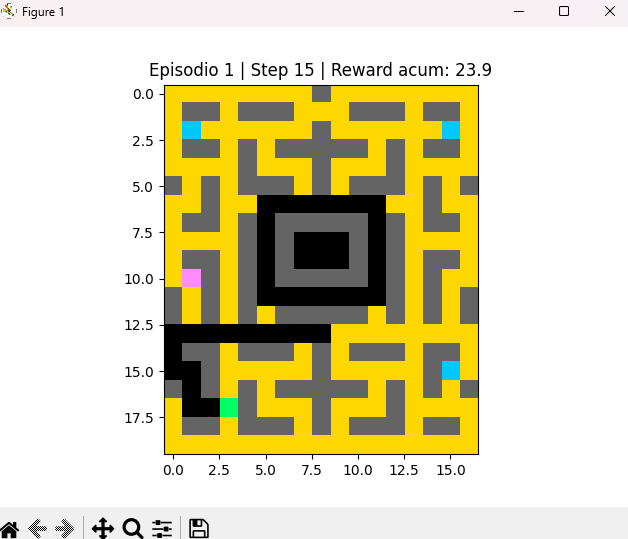
\includegraphics[width=0.5\textwidth]{./figs/agent_playing.png}
\caption{Agente entrenado jugando una partida de simulación}
\label{fig:agent_playing}
\end{figure}

Uno de los aspectos diferenciales del entorno \textit{SimplePacmanEnv} es la posibilidad de definir múltiples modos de observación. En función de la configuración seleccionada, el agente puede percibir desde una representación mínima del estado —por ejemplo, la posición relativa del agente y del fantasma— hasta observaciones más complejas que incluyen información adicional sobre el entorno, como la presencia de comodines, temporizadores o la distribución espacial de monedas. Esta flexibilidad convierte al entorno en una herramienta idónea para estudiar de forma sistemática la relación entre la complejidad del estado y el comportamiento del aprendizaje.

En los apartados siguientes se describen con mayor detalle las dinámicas del entorno, el comportamiento de los distintos elementos y la definición formal de los espacios de estados, acciones y recompensas.

\subsection{Motivación para implementar un entorno propio}

Una contribución clave de este trabajo es la implementación completa desde cero de un entorno tipo Pac-Man (\textit{SimplePacmanEnv}) en lugar de reutilizar entornos existentes. Aunque existen \textit{benchmarks} ampliamente utilizados en Aprendizaje por Refuerzo (por ejemplo, Atari o MiniGrid), en la mayoría de ellos el espacio de observaciones viene fijado por el propio entorno y no permite modificar de manera controlada el nivel de información accesible al agente sin alterar simultáneamente otros factores (dinámica, recompensas o reglas).

Dado que la pregunta de investigación de este TFM se centra en el efecto de la complejidad del estado observado, era imprescindible disponer de un entorno donde pudiera parametrizarse de forma explícita qué información recibe el agente, manteniendo constantes el resto de componentes del MDP. Esto motivó el desarrollo de un entorno propio, compatible con Gymnasium y Stable-Baselines3, que permite definir múltiples modos de observación (mínimo, comodín binario, temporizador y agregación espacial de monedas) sin modificar la dinámica del juego ni el sistema de recompensas.

Esta capacidad de control experimental no es trivial: requiere implementar desde cero la simulación del entorno (rejilla, colisiones, transiciones, recompensas, terminación de episodios), así como asegurar el cumplimiento estricto de la interfaz de Gymnasium para permitir entrenamientos reproducibles con librerías estándar. En consecuencia, el entorno desarrollado actúa como un \textit{benchmark} modular orientado específicamente a estudiar el compromiso entre simplicidad y expresividad en el diseño del estado.

\subsection{Espacio de estados y observaciones}

En el contexto del Aprendizaje por Refuerzo, el \textit{estado} representa la información que el agente utiliza para decidir su acción en cada paso temporal. En el entorno \textit{SimplePacmanEnv}, se distingue de manera explícita entre el estado completo del entorno y la \textit{observación} accesible al agente, siendo esta última el foco principal del análisis experimental.

El diseño del espacio de observaciones se ha realizado con el objetivo de permitir una modificación progresiva y controlada de la complejidad informacional, manteniendo constantes las dinámicas internas del entorno. De este modo, es posible evaluar cómo distintas representaciones del estado influyen en la velocidad de aprendizaje, la estabilidad del entrenamiento y el rendimiento final del agente.

Formalmente, el entorno se define sobre una rejilla bidimensional discreta. El estado completo incluye, entre otros elementos, la posición del agente, la posición del fantasma, la disposición de muros, la localización de monedas y el estado de posibles comodines. Sin embargo, no toda esta información es necesariamente observable por el agente en todas las configuraciones.

Se han definido varios \textbf{modos de observación}, cada uno de los cuales incrementa progresivamente la complejidad del estado observado:

\begin{itemize}
    \item \textbf{Observación mínima (Minimal):} el agente percibe únicamente su propia posición y la posición del fantasma dentro de la rejilla. Esta configuración proporciona una representación muy compacta del estado, pero omite información relevante sobre el entorno, como la localización de las monedas.
    
    \item \textbf{Observación con comodín binario (Power Boolean):} además de las posiciones del agente y del fantasma, se incluye una variable booleana que indica si un comodín se encuentra activo. Esta extensión introduce información contextual adicional sin aumentar significativamente la dimensionalidad del estado.
    
    \item \textbf{Observación con temporizador de comodín (Power Timer):} en este modo, la observación incorpora el tiempo restante de activación del comodín. Esta información permite al agente anticipar la duración de su ventaja temporal frente al fantasma, incrementando la complejidad y el carácter temporal del estado.
    
    \item \textbf{Observación con distribución de monedas (Coins Quadrants):} el entorno se divide en cuadrantes, y la observación incluye información agregada sobre la cantidad de monedas restantes en cada uno de ellos. Este enfoque introduce una representación espacial más rica del entorno sin recurrir a observaciones a nivel de celda.
    
    \item \textbf{Observación basada en imagen (opcional):} de forma experimental, se contempla un modo de observación en el que el estado se representa como una matriz o imagen que codifica directamente el contenido de cada celda del entorno. Este modo incrementa significativamente la dimensionalidad del estado y permite analizar el comportamiento de los algoritmos ante observaciones de tipo visual.
\end{itemize}

Cada uno de estos modos define un espacio de observaciones diferente, tanto en dimensionalidad como en contenido semántico. En particular, el aumento progresivo de información no implica necesariamente una mejora del aprendizaje: estados más complejos pueden introducir redundancia, ruido o dificultar la generalización, especialmente en algoritmos sensibles a la dimensionalidad del espacio de entrada.

Desde el punto de vista experimental, todos los modos de observación se implementan manteniendo invariables el espacio de acciones, la dinámica del entorno y la función de recompensa. Esta decisión de diseño garantiza que cualquier diferencia observada en el rendimiento de los agentes pueda atribuirse principalmente a la complejidad del estado observado y no a otros factores externos.

En los siguientes apartados se describen las dinámicas del entorno, el comportamiento del agente y del enemigo, así como el sistema de recompensas utilizado para guiar el aprendizaje.

\subsection{Espacio de acciones y dinámica del agente}

El comportamiento del agente en el entorno \textit{SimplePacmanEnv} se define a través de un espacio de acciones discreto y una dinámica determinista, diseñados con el objetivo de simplificar el análisis del aprendizaje y aislar el impacto de la representación del estado.

El espacio de acciones disponible para el agente está compuesto por un conjunto reducido de movimientos discretos, correspondientes a los desplazamientos en las cuatro direcciones cardinales:
\begin{itemize}
    \item Movimiento hacia arriba.
    \item Movimiento hacia abajo.
    \item Movimiento hacia la izquierda.
    \item Movimiento hacia la derecha.
\end{itemize}

En cada paso temporal, el agente selecciona una de estas acciones en función de su política actual. La acción se traduce en un intento de desplazamiento dentro de la rejilla del entorno. Si la celda de destino corresponde a un muro, la acción no tiene efecto y el agente permanece en su posición actual. En caso contrario, la posición del agente se actualiza de manera determinista.

Esta dinámica sencilla permite eliminar comportamientos estocásticos no controlados y facilita la interpretación de los resultados experimentales. De este modo, cualquier variación en el rendimiento del agente puede atribuirse principalmente a la política aprendida y a la información observacional disponible, en lugar de a fluctuaciones aleatorias del entorno.

Además del desplazamiento del agente, en cada paso temporal se actualiza el estado interno del entorno, incluyendo la posible recolección de monedas y la interacción con otros elementos, como el fantasma o los comodines. Estas actualizaciones se realizan de manera consistente e independiente del algoritmo de aprendizaje utilizado, garantizando un comportamiento homogéneo del entorno a lo largo de todos los experimentos.

Desde el punto de vista del aprendizaje, el agente no dispone de conocimiento previo sobre las reglas del entorno ni sobre las consecuencias de sus acciones. La política se construye progresivamente a partir de la experiencia acumulada, guiada únicamente por las recompensas recibidas tras cada transición. Esta configuración refuerza el carácter exploratorio del problema y sitúa el aprendizaje en un marco puramente basado en la interacción agente–entorno.

La simplicidad del espacio de acciones y de la dinámica del agente contribuye a que el foco experimental se sitúe en la complejidad del estado observado, evitando que la dificultad del problema venga dominada por factores externos como acciones continuas, ruido en las transiciones o comportamientos impredecibles del entorno.

\subsection{Comportamiento del fantasma}

Además del agente controlado por el algoritmo de Aprendizaje por Refuerzo, el entorno \textit{SimplePacmanEnv} incluye un segundo actor: un enemigo denominado \textit{fantasma}. La presencia de este elemento introduce una fuente de riesgo en el entorno, obligando al agente a equilibrar comportamientos exploratorios con estrategias de evitación.

El comportamiento del fantasma se ha diseñado de forma deliberadamente simple y controlada, con el objetivo de no introducir complejidad innecesaria en las dinámicas del entorno. En cada paso temporal, el fantasma ejecuta una acción de movimiento siguiendo una política predefinida, independiente del algoritmo de aprendizaje utilizado por el agente. De este modo, el comportamiento del enemigo es consistente a lo largo de todos los experimentos y no se adapta a la política del agente.

El espacio de acciones del fantasma coincide con el del agente, permitiendo desplazamientos discretos en las cuatro direcciones cardinales. Al igual que en el caso del agente, los movimientos están sujetos a las restricciones impuestas por los muros del entorno, de modo que el fantasma no puede atravesar paredes ni salir de los límites de la rejilla.

Dependiendo de la configuración del entorno, el movimiento del fantasma puede seguir una estrategia determinista simple, como desplazarse hacia la posición del agente, o una política estocástica limitada, seleccionando acciones válidas de manera aleatoria. Esta flexibilidad permite introducir distintos niveles de dificultad sin alterar la estructura general del entorno ni la función de recompensa.

La interacción entre el agente y el fantasma constituye uno de los principales mecanismos de terminación del episodio. Si el agente colisiona con el fantasma en una celda compartida, el episodio finaliza inmediatamente y se aplica una penalización significativa en la recompensa. Este evento incentiva al agente a desarrollar comportamientos evasivos y a planificar sus movimientos teniendo en cuenta la posición relativa del enemigo.

El diseño del fantasma como un elemento externo con comportamiento fijo permite centrar el análisis experimental en la capacidad del agente para utilizar la información observacional disponible. De este modo, se evita que la complejidad del problema venga dominada por interacciones adversarias dinámicas, manteniendo el foco en la relación entre la representación del estado y el proceso de aprendizaje.

\subsection{Sistema de recompensas}

El sistema de recompensas constituye el principal mecanismo mediante el cual el agente recibe retroalimentación sobre la calidad de sus acciones y, por tanto, desempeña un papel fundamental en el proceso de aprendizaje. En el entorno \textit{SimplePacmanEnv}, la función de recompensa se ha diseñado cuidadosamente para incentivar comportamientos deseables y penalizar situaciones adversas, manteniendo al mismo tiempo un equilibrio que evite soluciones triviales o inestables.

El objetivo principal del agente es maximizar la recompensa acumulada mediante la recolección de monedas distribuidas en el entorno, al tiempo que evita la colisión con el fantasma. Para ello, el sistema de recompensas se compone de los siguientes elementos:

\begin{itemize}
    \item \textbf{Recompensa por recolección de monedas:} cada vez que el agente recoge una moneda, recibe una recompensa positiva. Este refuerzo incentiva la exploración del entorno y guía al agente hacia las zonas con mayor densidad de recompensas.
    
    \item \textbf{Penalización por colisión con el fantasma:} si el agente entra en la misma celda que el fantasma, el episodio finaliza y se aplica una penalización negativa significativa. Esta señal refuerza comportamientos evasivos y promueve una planificación más cuidadosa de las acciones.
    
    \item \textbf{Penalización por paso temporal:} en cada paso del episodio se aplica una pequeña penalización constante. Este término evita que el agente adopte estrategias pasivas o cíclicas, incentivando la resolución eficiente del episodio en el menor número de pasos posible.
    
    \item \textbf{Recompensa por finalización exitosa del episodio:} cuando el agente logra recolectar todas las monedas del entorno, el episodio finaliza con una recompensa adicional que refuerza el objetivo global de la tarea.
\end{itemize}

La magnitud relativa de estas recompensas ha sido seleccionada de forma empírica para asegurar un equilibrio adecuado entre exploración, seguridad y eficiencia. Penalizaciones excesivamente severas pueden dificultar el aprendizaje al desalentar la exploración, mientras que recompensas demasiado elevadas pueden provocar comportamientos miopes centrados en objetivos inmediatos.

Un aspecto relevante del diseño es que la función de recompensa se mantiene idéntica para todas las configuraciones de observación y para todos los algoritmos evaluados. Esta decisión garantiza que cualquier diferencia observada en el rendimiento de los agentes pueda atribuirse a la complejidad del estado observado o al algoritmo de aprendizaje utilizado, y no a variaciones en la señal de refuerzo.

En conjunto, este sistema de recompensas proporciona una señal de aprendizaje clara y coherente con los objetivos del entorno, permitiendo evaluar de forma consistente cómo distintas representaciones del estado influyen en la capacidad del agente para aprender políticas eficaces.

\subsection{Condiciones de terminación de los episodios}

Las condiciones de terminación determinan cuándo finaliza un episodio de interacción entre el agente y el entorno, y desempeñan un papel relevante tanto en la estabilidad del aprendizaje como en la interpretación de las métricas de evaluación. En el entorno \textit{SimplePacmanEnv}, los episodios se han definido de forma que reflejen situaciones naturales de éxito o fracaso, manteniendo al mismo tiempo una duración acotada.

Un episodio puede finalizar bajo cualquiera de las siguientes condiciones:

\begin{itemize}
    \item \textbf{Finalización exitosa:} el agente ha recolectado todas las monedas presentes en el entorno. Este caso representa el cumplimiento completo del objetivo de la tarea y se acompaña de una recompensa positiva adicional.
    
    \item \textbf{Colisión con el fantasma:} el agente entra en la misma celda que el fantasma. Esta situación se considera un fallo y provoca la finalización inmediata del episodio con la correspondiente penalización.
    
    \item \textbf{Límite máximo de pasos:} si el agente supera un número máximo predefinido de pasos sin alcanzar el objetivo, el episodio finaliza automáticamente. Esta condición evita episodios excesivamente largos y comportamientos cíclicos que no conducen a una solución.
\end{itemize}

El establecimiento de un límite máximo de pasos resulta especialmente relevante para garantizar la comparabilidad entre experimentos. Sin esta restricción, los agentes podrían prolongar indefinidamente los episodios, dificultando la interpretación de métricas como la recompensa acumulada o la duración media de los episodios.

Al igual que ocurre con el resto de elementos del entorno, las condiciones de terminación se mantienen constantes para todas las configuraciones de observación y para todos los algoritmos de aprendizaje evaluados. De este modo, se asegura que las diferencias observadas en el rendimiento de los agentes se deban a la representación del estado o al algoritmo utilizado, y no a variaciones en la definición del episodio.

En conjunto, estas condiciones de terminación contribuyen a un marco experimental bien definido y controlado, facilitando el análisis comparativo del aprendizaje y la obtención de conclusiones reproducibles.

\section{Algoritmos de aprendizaje por refuerzo utilizados}

\subsection{Configuración común de entrenamiento}

Para garantizar la comparabilidad de los resultados obtenidos con los distintos algoritmos de Aprendizaje por Refuerzo (DQN, A2C y PPO), se ha establecido una configuración común de entrenamiento que se aplica de forma uniforme en todos los experimentos. Esta configuración incluye los parámetros generales del entrenamiento, la infraestructura utilizada para la ejecución de los experimentos y el protocolo de evaluación.

Los principales aspectos comunes a todos los experimentos son los siguientes:

\begin{itemize}
    \item \textbf{Entorno de entrenamiento:} todos los algoritmos han sido entrenados en el entorno \textit{SimplePacmanEnv} descrito anteriormente, utilizando el modo de observación seleccionado en cada experimento (ya sea mínimo, con comodín binario, temporizador de poder, o distribución de monedas).
    
    \item \textbf{Parámetros de entrenamiento:} se ha utilizado un conjunto común de hiperparámetros para los tres algoritmos, con variaciones específicas que se detallarán más adelante para cada algoritmo. Los parámetros incluyen la tasa de aprendizaje, el tamaño del batch, el tamaño del buffer de experiencias y la frecuencia de actualización de la red.
    
    \item \textbf{Número de pasos de entrenamiento:} el número de pasos de entrenamiento ha sido de 1 millón de pasos por defecto, salvo en algunas configuraciones específicas, como las pruebas de exhaustividad con 2 millones de pasos para A2C. El entrenamiento se ha ejecutado utilizando un criterio de parada temprana, que detiene el entrenamiento si no hay mejoras sustanciales en la política aprendida durante un número definido de evaluaciones consecutivas sin mejora.
    
    \item \textbf{Evaluación del agente:} para evaluar el rendimiento del agente durante el entrenamiento, se ha implementado un protocolo de evaluación cada 50,000 pasos de entorno, ejecutando múltiples episodios para calcular el rendimiento medio. Además, se ha utilizado una evaluación adicional al final de cada entrenamiento para validar el modelo entrenado.
    
    \item \textbf{Optimización de hiperparámetros:} inicialmente, los hiperparámetros fueron ajustados manualmente a través de pruebas y errores. Posteriormente, se utilizó la librería Optuna para realizar una búsqueda más sistemática de los mejores valores para parámetros como la tasa de aprendizaje, el tamaño del batch y otros parámetros relevantes para la estabilidad del aprendizaje.
\end{itemize}

Esta configuración común garantiza que las diferencias observadas entre los algoritmos no sean el resultado de una variabilidad en la configuración del entorno o en los parámetros de entrenamiento, sino que puedan atribuirse a las características específicas de cada algoritmo de Aprendizaje por Refuerzo.

En los siguientes apartados se describirán las configuraciones particulares de cada algoritmo (DQN, A2C y PPO), incluyendo los detalles adicionales que corresponden a cada uno de ellos, como la arquitectura de la red neuronal utilizada, los métodos de exploración y explotación, y los mecanismos de actualización de la política.

\subsection{Entrenamiento con Deep Q-Network (DQN)}

El algoritmo \textit{Deep Q-Network} (DQN) se ha utilizado en este trabajo como representante de los métodos de Aprendizaje por Refuerzo basados en valor. DQN es especialmente adecuado para entornos con espacios de acción discretos, como el entorno \textit{SimplePacmanEnv}, donde el agente debe seleccionar una acción entre un conjunto finito de movimientos posibles.

En esta implementación, el agente DQN aprende una aproximación de la función de acción-valor $Q(s,a)$ mediante una red neuronal profunda. Dicha red recibe como entrada la observación del estado definida por el modo de observación seleccionado y produce como salida un valor estimado para cada acción disponible. La política seguida durante el entrenamiento es una política $\epsilon$-greedy, que equilibra exploración y explotación permitiendo al agente seleccionar acciones aleatorias con una probabilidad decreciente a lo largo del entrenamiento.

El proceso de entrenamiento se basa en la interacción repetida del agente con el entorno, almacenando las transiciones $(s, a, r, s')$ en un buffer de experiencias. Estas transiciones se muestrean de forma aleatoria para actualizar la red neuronal, reduciendo la correlación temporal entre muestras y mejorando la estabilidad del aprendizaje. Para evitar oscilaciones en la estimación de la función de valor, se emplea una red objetivo (\textit{target network}) que se actualiza de forma periódica con los parámetros de la red principal.

Los principales hiperparámetros utilizados en el entrenamiento con DQN incluyen la tasa de aprendizaje, el tamaño del buffer de experiencias, el tamaño del batch de entrenamiento, el factor de descuento $\gamma$ y la frecuencia de actualización de la red objetivo. Estos parámetros influyen de manera significativa en la estabilidad y velocidad de convergencia del algoritmo, especialmente en entornos donde la observación del estado puede variar en complejidad y dimensionalidad.

Debido a la naturaleza secuencial del aprendizaje y al elevado número de interacciones necesarias para que DQN converja hacia una política estable, el coste computacional de este algoritmo resulta considerable en comparación con métodos actor-crítico. Por este motivo, el número de experimentos exhaustivos realizados con DQN fue limitado en relación con A2C y PPO, priorizando configuraciones representativas que permitieran analizar tendencias generales sin incurrir en tiempos de ejecución excesivos.

El rendimiento del agente DQN se evalúa de forma periódica durante el entrenamiento mediante episodios de prueba independientes, lo que permite monitorizar la evolución de la política aprendida y detectar posibles problemas de inestabilidad o sobreajuste. Estas evaluaciones proporcionan una referencia objetiva para comparar el comportamiento de DQN con el de los demás algoritmos considerados en el estudio.

\subsection{Entrenamiento con Advantage Actor-Critic (A2C)}

El algoritmo \textit{Advantage Actor-Critic} (A2C) se ha empleado en este trabajo como representante de los métodos actor-crítico, que combinan el aprendizaje de una política parametrizada con la estimación del valor de los estados. A diferencia de los métodos basados exclusivamente en valor, como DQN, A2C resulta más flexible ante variaciones en la dimensionalidad del espacio de observación y presenta una mayor estabilidad en entornos con dinámicas complejas.

En A2C, el proceso de aprendizaje se basa en dos componentes principales: un \textit{actor}, encargado de aprender la política $\pi_\theta(a|s)$, y un \textit{crítico}, que estima la función de valor $V_\phi(s)$. El crítico proporciona una señal de error denominada \textit{ventaja} (\textit{advantage}), que mide cuánto mejor resulta ejecutar una acción concreta respecto al valor esperado del estado. Esta señal se utiliza para actualizar la política del actor, reduciendo la varianza del gradiente y mejorando la estabilidad del aprendizaje.

Una de las características distintivas de A2C es el uso de múltiples entornos ejecutados en paralelo durante el entrenamiento. En cada iteración, el agente interactúa simultáneamente con varias instancias del entorno \textit{SimplePacmanEnv}, recopilando trayectorias que se utilizan para actualizar la política de forma síncrona. Este enfoque permite acelerar el aprendizaje y mitigar los efectos negativos de correlación temporal entre muestras consecutivas.

En el contexto de este trabajo, el algoritmo A2C se ha entrenado utilizando arquitecturas de red neuronal compartidas para el actor y el crítico, con capas ocultas densas que procesan la observación del estado en función del modo de observación seleccionado. Los hiperparámetros clave del entrenamiento incluyen la tasa de aprendizaje, el número de pasos por actualización, el coeficiente de entropía y el factor de descuento $\gamma$. El coeficiente de entropía desempeña un papel relevante al fomentar la exploración, evitando una convergencia prematura hacia políticas deterministas subóptimas.

A diferencia de DQN, A2C no requiere una memoria explícita de experiencias ni el uso de redes objetivo, lo que reduce la complejidad de la implementación y el consumo de memoria. Estas características hacen que A2C resulte computacionalmente más eficiente y adecuado para la ejecución de experimentos a gran escala, como la optimización exhaustiva de hiperparámetros realizada en este trabajo.

Debido a su equilibrio entre estabilidad, eficiencia y capacidad de adaptación a distintos espacios de observación, A2C ha sido uno de los algoritmos principales en el estudio experimental. Se han realizado múltiples ejecuciones con distintas configuraciones de hiperparámetros y modos de observación, permitiendo analizar de forma detallada cómo la complejidad del estado influye en el proceso de aprendizaje y en el rendimiento final del agente.

\subsection{Entrenamiento con Proximal Policy Optimization (PPO)}

El algoritmo \textit{Proximal Policy Optimization} (PPO) ha sido seleccionado en este trabajo debido a su robustez y simplicidad en comparación con otros métodos actor-crítico, como A3C o TRPO (Trust Region Policy Optimization). PPO es una de las técnicas más utilizadas en la práctica de Aprendizaje por Refuerzo Profundo, ya que ofrece un buen equilibrio entre rendimiento y facilidad de implementación.

PPO mejora sobre los métodos actor-crítico tradicionales mediante el uso de una técnica llamada \textit{clipping}, que limita la magnitud de las actualizaciones de la política, evitando cambios drásticos que podrían desestabilizar el entrenamiento. Este método introduce un término adicional en la función de pérdida que penaliza las actualizaciones de la política que se alejan demasiado de la anterior, lo que se expresa de la siguiente manera:

\begin{equation}
L^{CLIP}(\theta) = \mathbb{E}\left[\min\left(r_t(\theta)A_t, \text{clip}(r_t(\theta), 1 - \epsilon, 1 + \epsilon)A_t\right)\right],
\end{equation}

donde $r_t(\theta)$ es la razón entre la probabilidad de acción de la nueva política y la anterior, y $A_t$ es el valor de la ventaja en el paso temporal $t$. El parámetro $\epsilon$ controla el rango dentro del cual se permite la actualización, y su valor es una constante que equilibra la estabilidad y la capacidad de adaptación de la política.

Una de las principales ventajas de PPO es su capacidad para adaptarse de forma eficiente a diferentes entornos y arquitecturas. A diferencia de TRPO, que requiere cálculos costosos de la matriz Hessiana para cada actualización, PPO emplea una aproximación más simple, basada en el clipping de la probabilidad de acción. Esto reduce significativamente la complejidad computacional, haciendo que PPO sea más fácil de implementar y más rápido de entrenar, lo que lo convierte en un algoritmo ideal para entornos con recursos limitados o experimentos a gran escala.

El entrenamiento con PPO se ha realizado utilizando una red neuronal de política con arquitectura de capas densas, similar a la utilizada en A2C, con un tamaño de batch mayor y una mayor frecuencia de actualizaciones. El uso de \textit{VecNormalize} para normalizar las observaciones y las recompensas ha sido una de las claves para mejorar la estabilidad y eficiencia del algoritmo, permitiendo que el agente se adapte de manera más rápida y confiable a las distintas configuraciones del entorno.

PPO es conocido por su robustez ante cambios en la complejidad del estado, por lo que se ha seleccionado como uno de los algoritmos principales en este trabajo. Al igual que A2C, PPO ha sido entrenado en paralelo utilizando múltiples instancias del entorno para acelerar el proceso de aprendizaje. Además, como en los otros algoritmos, se ha empleado una estrategia de parada temprana para evitar el sobreajuste y asegurar que el modelo entrenado no se desvíe de una solución óptima.

En resumen, PPO se distingue por su simplicidad, eficiencia y estabilidad, características que lo convierten en el algoritmo ideal para comparar cómo diferentes representaciones del estado afectan al rendimiento del agente. En los siguientes apartados se presentarán los resultados obtenidos con PPO, los cuales servirán como base para las comparaciones entre los distintos algoritmos estudiados en este trabajo.

